% -- Encoding UTF-8 without BOM
% -- XeLaTeX => PDF (BIBER)

\documentclass[]{cv-style}          % Add 'print' as an option into the square bracket to remove colours from this template for printing. 
                                    % Add 'espanol' as an option into the square bracket to change the date format of the Last Updated Text

\sethyphenation[variant=british]{english}{} % Add words between the {} to avoid them to be cut 
\usepackage{graphicx}

\begin{document}

\header{Flores}{ Facundo Gabriel}           % Your name
\lastupdated

%----------------------------------------------------------------------------------------
%	SIDEBAR SECTION  -- In the aside, each new line forces a line break
%----------------------------------------------------------------------------------------

\begin{aside}
%
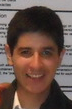
\includegraphics[width=0.5\textwidth]{profile.png}
\section{Contacto}
Bº Ciudad Valdivia
Mza. 751 "A" Casa Nº 3
Salta, Argentina
~
+54 (387) 495 1508
+54 (387) 462 2866
~
flores.facundogabriel
@gmail.com
~
linkedin/facundogflores
github/facundogflores
%
\section{Idiomas}
Español (Nativo)
Inglés (Alto)
%
\section{Programación}
%{\color{red} $\varheartsuit$} 
C, C++, Python, Java, Php, C\#
SQL, HTML, CSS
%\LaTeX{}
%
\section{Sistemas Operativos}
 Linux, Free-Bsd, Windows
%
\section{Herramientas}
 GIT, SVN, Cmake, GCC, GDB
%
\section{Editores}
 VIM, Atom
%
\end{aside}

%----------------------------------------------------------------------------------------
%	EDUCATION SECTION
%----------------------------------------------------------------------------------------

\section{Educación}

\begin{entrylist}
%------------------------------------------------
\entry
{2009--2013}
{Computador Universitario}
{Universidad Nacional de Salta}
{\jobtitle{,}
\begin{itemize}
\item Desarrollo de una librería utilizando CUDA para la resolución de sistemas de ecuaciones lineales a gran escala.
\item C++, CUDA.
\end{itemize}}

{\vspace{-0.3cm}}
\end{entrylist}
%------------------------------------------------
%----------------------------------------------------------------------------------------
%	WORK EXPERIENCE SECTION
%----------------------------------------------------------------------------------------

\section{Experiencia}

\begin{entrylist}
%------------------------------------------------
\entry
  {2015-2016}
  {Desarrollador Web PHP}
  {DIGIO S.R.L}
  {\jobtitle{Full Stack}\\ 
  \begin{itemize}
    \item PHP, Postgres, Codeigniter
    \item MVC
    \item Generación de Reportes
  \end{itemize}}
  
 \entry
  {2015}
  {Informática Aplicada}
  {UNSA - Fac. Cs. de la Saluda}
  {\jobtitle{Jefe de Trabajos Prácticos}\\ 
  \begin{itemize}
    \item MS Office
    \item Excel Avanzado
    \item SPSS
  \end{itemize}}
  
\entry
  {2014-2015}
  {Paradigmas y Lenguajes }
  {UNSA - Fac. Cs. Exactas}
  {\jobtitle{Auxiliar Docente de 2º Categoría}\\ 
  \begin{itemize}
    \item Uso de paradigmas de programación: Estructurado, POO, Funcional, Concurrente y Paralelo.
    \item C++, Python, Java
    \item POSIX
    \item OpenMP, CUDA
  \end{itemize}}


%------------------------------------------------

\end{entrylist}


%----------------------------------------------------------------------------------------
%	SKILLS SECTION
%----------------------------------------------------------------------------------------

\section{Habilidades}
  \vspace{-0.2cm}

Excelente comunicación y trabajo en equipo. Proactivo y autodidacta. 



%----------------------------------------------------------------------------------------
%	OTHER QUALIFICATIONS SECTION
%----------------------------------------------------------------------------------------

%\section{other qualifications}

%\begin{entrylist}
%------------------------------------------------
%\entry
%{2013}
%{Leadership}
%{Institution}
%{\vspace{-0.3cm}}
%------------------------------------------------
%\entry
%{2011}
%{Qualification}
%{Institution}
%{\vspace{-0.3cm}}
%------------------------------------------------
%\end{entrylist}

%----------------------------------------------------------------------------------------
%	AWARDS SECTION
%----------------------------------------------------------------------------------------
\section{Premios}

\begin{entrylist}
%------------------------------------------------
\entry
{2013}
{Alumno destacado - Tarjeta Gráfica NVIDIA GTX 480}
{Escuela de Computación de Alto Rendimiento. NVIDIA Fellow: Dr. Manuel Ujaldón}
{}
%------------------------------------------------
\end{entrylist}

\section{Cursos}

\begin{entrylist}
%------------------------------------------------
\entry
{2013}
{Módulo GPGPU CUDA - Dr. Manuel Ujaldón}
{II Escuela de Computación de Alto Rendimiento}
{}
%------------------------------------------------
\end{entrylist}

\begin{entrylist}
%------------------------------------------------
\entry
{2012}
{Ethical Hacking}
{JUCSE - Universidad Católica de Santiago del Estero}
{}
%------------------------------------------------
\end{entrylist}

\begin{entrylist}
%------------------------------------------------
\entry
{2011}
{Taller de Android - Ing. Manuel Moscoso}
{Universidad Nacional de Salta}
{}
%------------------------------------------------
\end{entrylist}

\begin{entrylist}
%------------------------------------------------
%------------------------------------------------
\end{entrylist}

%----------------------------------------------------------------------------------------
%	INTERESTS SECTION
%----------------------------------------------------------------------------------------

%----------------------------------------------------------------------------------------

\end{document}